\documentclass[12pt,aspectratio=169,xcolor=dvipsnames]{beamer}
\usetheme[pageofpages=of,% String used between the current page and the
                         % total page count.
          bullet=circle,% Use circles instead of squares for bullets.
          titleline=true,% Show a line below the frame title.
          alternativetitlepage=true,% Use the fancy title page.
          ]{Torino}

\usecolortheme{iiia}

\usepackage{libertine}

% definitions

\newcommand{\wrt}{\textit{wrt}}

\newcommand{\titleicon}[2]{%
\makebox[\framewidth]{#1\hfill\raisebox{-0.25ex}{\includegraphics[height=5mm]{img/icons/#2}}}%
}

\newcommand{\icon}[1]{%
\mathord{\raisebox{-0.25ex}{\includegraphics[height=2ex]{#1}}}%
}

\newcommand{\inline}[1] {%
\mathord{\raisebox{-0.5ex}{\includegraphics[height=2.5ex]{img/#1}}}%
}

\makeatletter
\newcommand*{\shiftbox}[2]{%
    \settowidth{\@tempdima}{#2}%
    \makebox[\@tempdima]{\hspace*{#1}#2}%
}
\makeatother

% dashed box

\usepackage{environ}

\NewEnviron{dashedbox}{
    \par
    \begin{tikzpicture}
        \node[rectangle,minimum width=0.9\textwidth] (m) {\begin{minipage}{0.85\textwidth}\BODY\end{minipage}};
        \draw[dashed] (m.south west) rectangle (m.north east);
    \end{tikzpicture}
}

% don't use ugly monospace font for URLs

\urlstyle{same}

% contour text

\usepackage[outline]{contour}

% use title field

\usepackage{authoraftertitle}

% euro symbol

\usepackage[official]{eurosym}

% use Font Awesome icons

\usepackage{fontawesome}

% comment

\usepackage{comment}

% tikz

\usepackage{tikz}
\usepackage{varwidth}
\usetikzlibrary{calc,fit,positioning,shapes}
\usetikzlibrary{decorations.pathreplacing,calc}
\usetikzlibrary{arrows,arrows.meta} % Stealth
\usetikzlibrary{overlay-beamer-styles} % alt
\tikzstyle{label_side}=[anchor=west,align=left,xshift=1mm,font=\scriptsize]
\tikzstyle{label_below}=[anchor=north,align=center,yshift=-5mm,font=\small]
\tikzstyle{label_above}=[anchor=base,align=center,yshift=2mm,font=\small]


\author{\raisebox{-7mm}{\Large\textbf{1\textsuperscript{st} Crash Course on Parallelization}}}
\title{\raisebox{5mm}{\textbf{Filippo Bistaffa}}}

\date{14 November 2023}

\begin{document}

\begin{frame}[t,plain]
    \titlepage
\end{frame}

\begin{frame}<{1,2}>[label=types]
    \frametitle{\titleicon{Types of Parallelization}{cpu}}
    \begin{figure}
        \begin{tikzpicture}[
            xscale=5,
            only1/.style = {alt=<1>{opacity=1}{opacity=0.2}},
            only123/.style = {alt=<{1,2,3}>{opacity=1}{opacity=0.2}},
            only124/.style = {alt=<{1,2,4}>{opacity=1}{opacity=0.2}},
        ]
            \def\photosize{3.5cm}
            \node[only123,outer sep=3mm,circle,draw,minimum size=\photosize,path picture={
                \node at (path picture bounding box.center){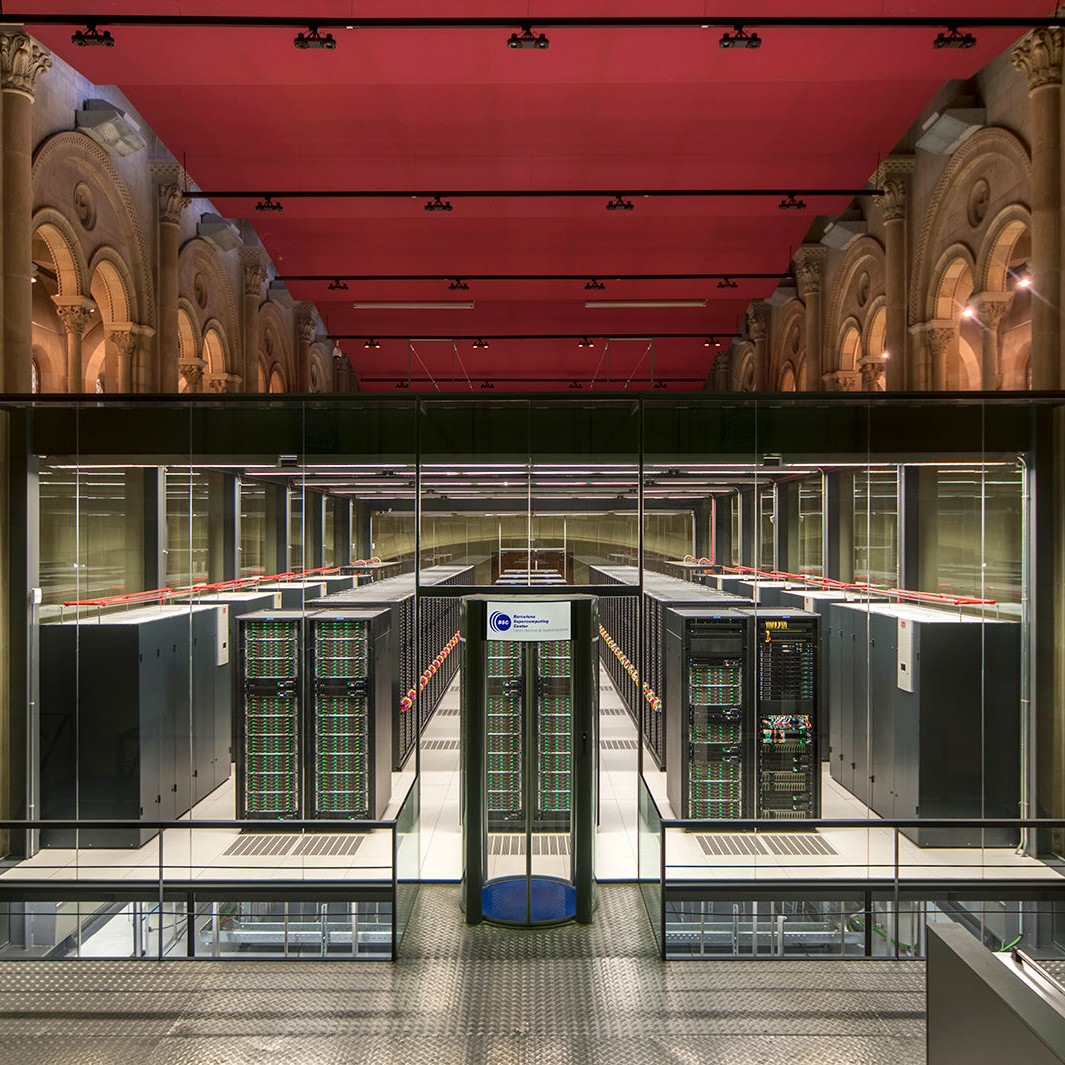
\includegraphics[width=\photosize]{img/marenostrum}};
            }] at (-1.5,0) (cluster) {};
            \node[only123,anchor=north,align=center] at (cluster.south) {Cluster};
            \node[only124,outer sep=3mm,circle,draw,minimum size=\photosize,path picture={
                \node at (path picture bounding box.center){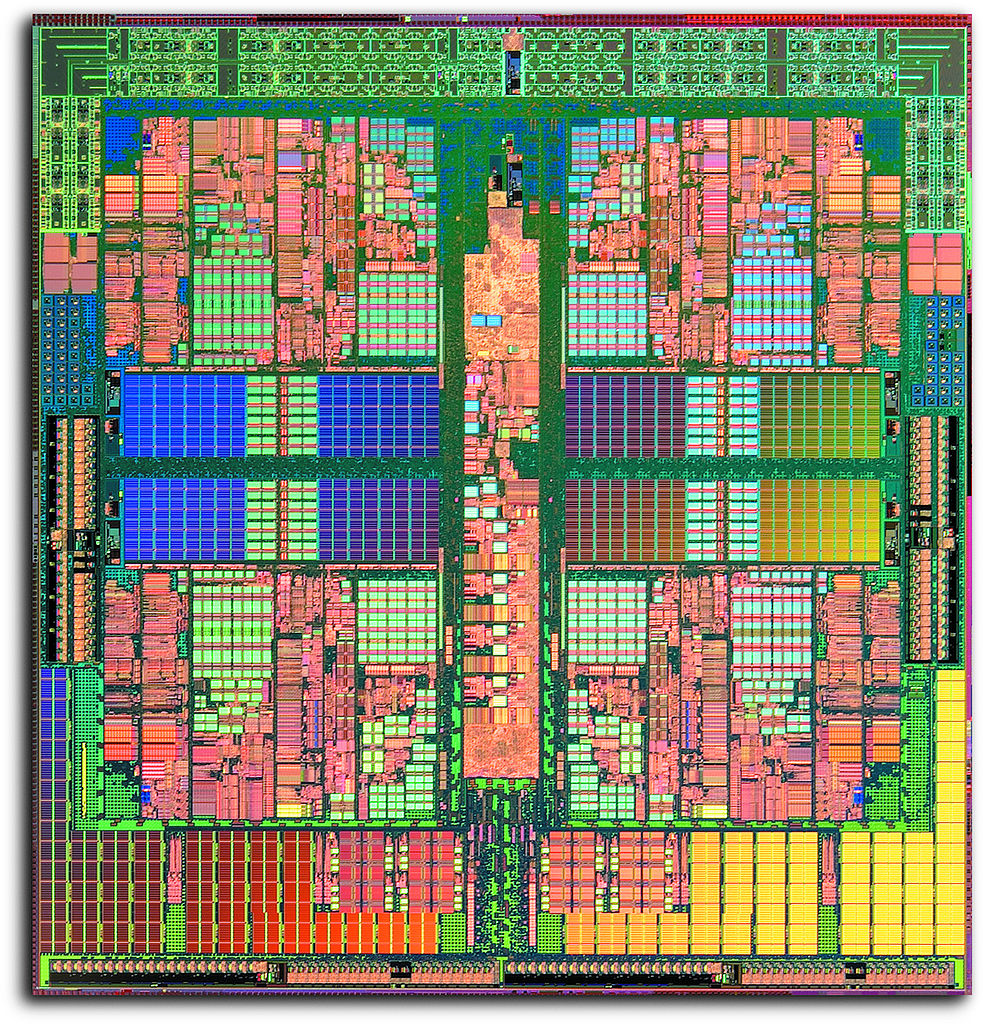
\includegraphics[width=\photosize]{img/multicore}};
            }] at (-0.5,0) (multicore) {};
            \node[only124,anchor=north,align=center] at (multicore.south) {Multi-Core};
            \node[only1,outer sep=3mm,circle,draw,minimum size=\photosize,path picture={
                \node at (path picture bounding box.center){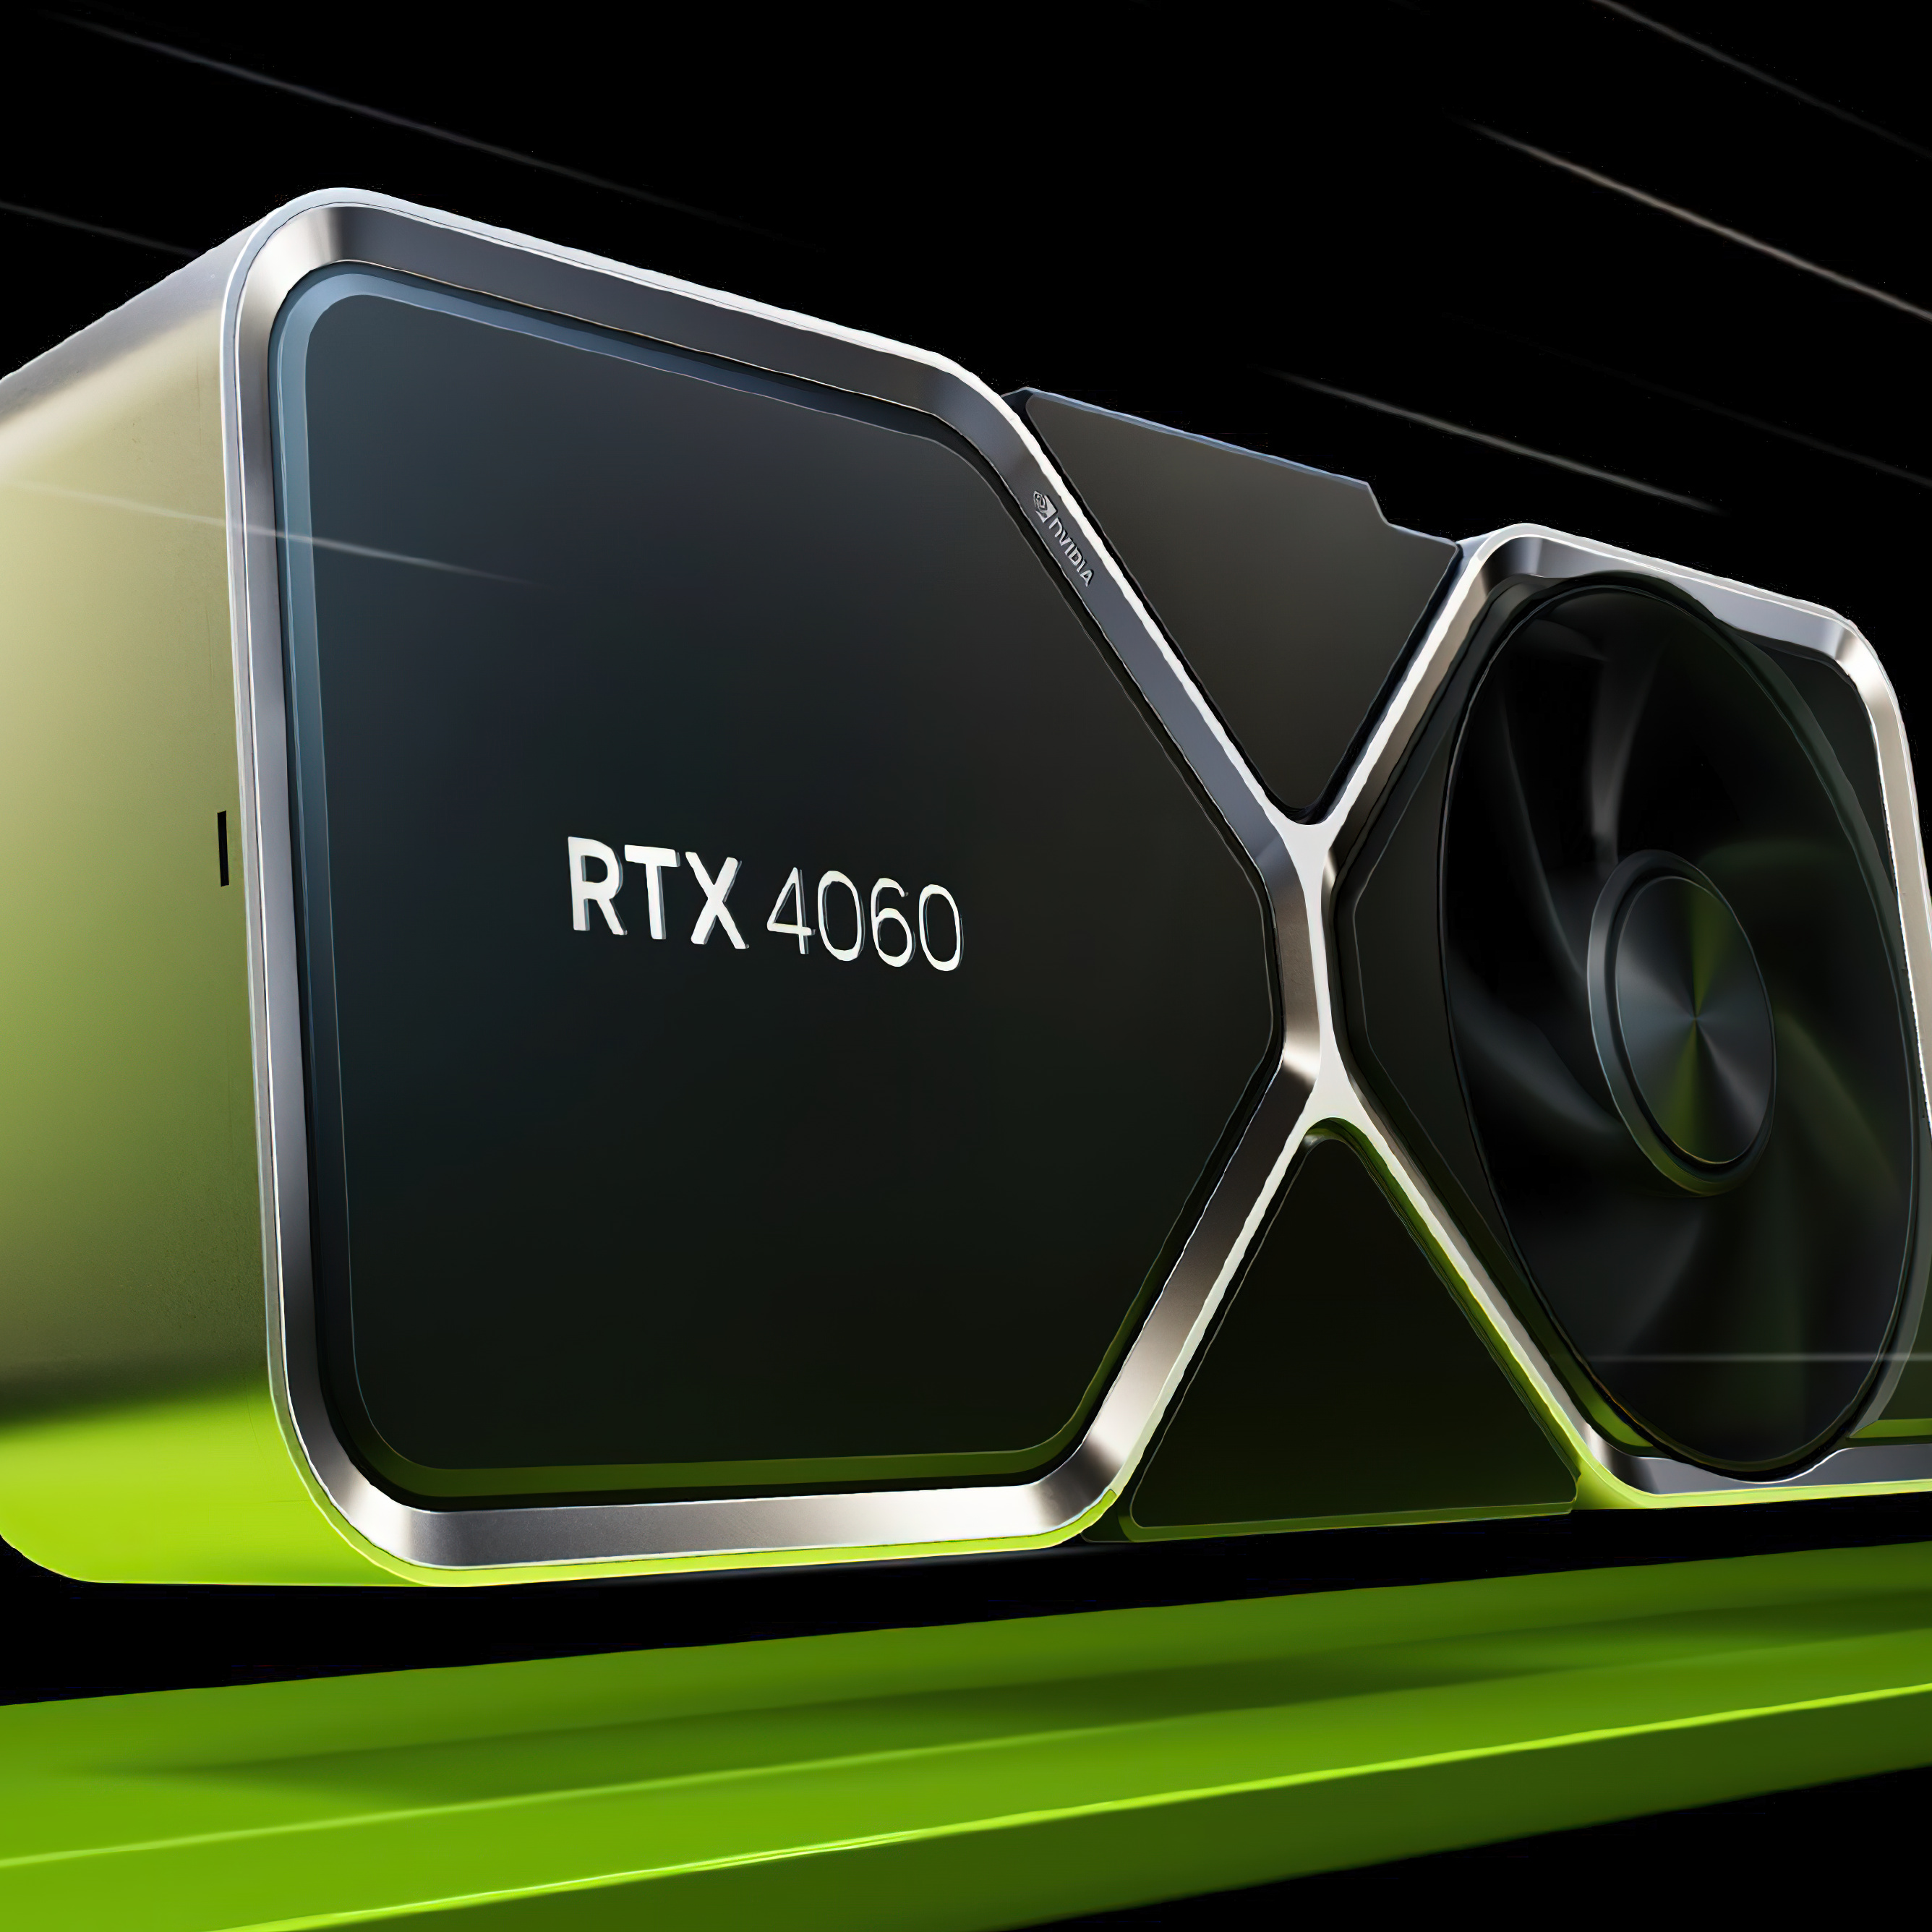
\includegraphics[width=\photosize]{img/nvidia}};
            }] at (0.5,0) (gpu) {};
            \node[only1,anchor=north,align=center] at (gpu.south) {GPU};
        \end{tikzpicture}
    \end{figure}
\end{frame}

\section{Cluster Parallelization}

\againframe<3>{types}

\begin{frame}{\titleicon{Local Software Execution}{workstation}}
    \begin{figure}
        \begin{tikzpicture}[xscale=5]
            \node at (+1.3,0) {};
            \node at (-1.3,0) {};
            \node[outer sep=3mm] at (-1,0) (u) {
\includegraphics[height=2cm]{img/icons/user}};
            \node[outer sep=3mm] at (+0,0) (s) {
\includegraphics[height=2cm]{img/icons/software}};
            \node[outer sep=3mm] at (+1,0) (w) {
\includegraphics[height=2cm]{img/icons/workstation}};
            \draw[thick,-{Stealth}] (u) -- (s);
            \draw[thick,-{Stealth}] (s) -- (w);
        \end{tikzpicture}
    \end{figure}
\end{frame}

\begin{frame}{\titleicon{Cluster Software Execution}{cluster}}
    \begin{figure}
        \begin{tikzpicture}[xscale=5]
            \node at (+1.3,0) {};
            \node at (-1.3,0) {};
            \node[outer sep=3mm] at (-1,0) (u) {
\includegraphics[height=2cm]{img/icons/user}};
            \node[outer sep=3mm] at (+0,0) (s) {
\includegraphics[height=2cm]{img/icons/software}};
            \node[outer sep=3mm] at (+1,0) (c) {
\includegraphics[height=2cm]{img/icons/cluster}};
            \draw[thick,-{Stealth}] (u) -- (s);
            \draw[thick,-{Stealth}] (s) -- (c);
            \node[outer sep=3mm] at ($(s.east)!0.5!(c.west)$) {
\includegraphics[height=5mm]{img/icons/forbidden}};
        \end{tikzpicture}
    \end{figure}
\end{frame}

\section{Multi-Core Parallelization}

\againframe<4>{types}

\end{document}
